\section{VM Placement Simulator}
\label{sec:injector}

The aim of \vmps is twofold:~(i) to relieve researchers of the burden of
dealing with VM creations and workload fluctuations when they evaluate
new VM placement algorithms and (ii) to offer the possibility to
compare them.
%
% The purpose of \vmps is to deliver a generic tool to evaluate new VM
% placement algorithms and offer the possibility to compare
% them. Concretely, it supports the management of VM creations and
% workload fluctuations.
% % as well as node apparitions/removals.
%  Researchers can
% thus focus on the implementation of new placement algorithms and
% evaluate how they behave in the presence of changes that occur during
% the simulation.
%
% In the following we give an overview of \vmps and describe its
% general functioning.

\subsubsection{Overview.}
\label{sec:overview}

\vmps has been implemented in Java by leveraging the \sg MSG API.
Although Java has an impact on the efficiency
of \sg, we believe its use is acceptable because Java offers important
benefits to researchers for the implementation of advanced scheduling
strategies, notably concerning the ease of implementation of new
strategies. As examples, we implemented the Snooze proposal in Java
and the DVMS proposal using Scala and Java.

\begin{wrapfigure}{r}{.48\linewidth}
\centering
\vspace*{-.6cm}
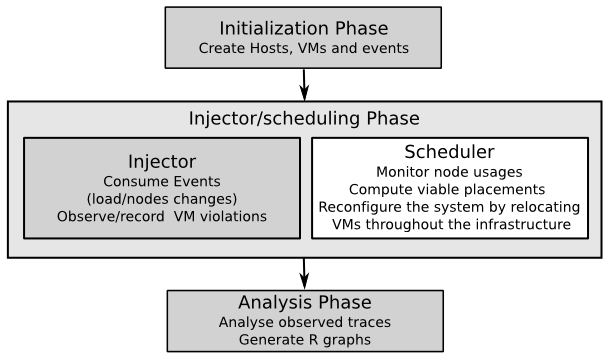
\includegraphics[width=.99\linewidth]{figures/VMPlaceS-workflow.pdf}
\vspace*{-.5cm}
\caption{\vmps's Workflow}
\flushleft \scriptsize{Gray parts correspond to the generic code while the white one
  must be provided by end-users. %The current version is released with
%  three different schedulers (centralized/hierarchical and
%  distributed).
}
\vspace*{-.8cm}
\label{fig:workflow}
\end{wrapfigure}
%
% From a high-level view,
\vmps performs a simulation in three phases, see
Fig.~\ref{fig:workflow}: (i) initialization, (ii) injection and (iii)
trace analysis.  The initialization phase corresponds to the creation
of the environment, the VMs and the generation of an event queue.
%
The simulation is performed by at least two \sg processes, one
executing the \emph{injector}, the generic part of the framework which
is in charge of injecting the events during the execution of the
simulation, and a second one executing the to-be-simulated
\emph{scheduling algorithm}.
%During the simulation the scheduling
%strategy is evaluated by injecting scheduling-relevant events.
%\AL[MS]{This sentence above is not accurate enough I? previously it
 % was : The
%\emph{injector} constitutes the generic part of the framework. It
%njects scheduling-relevant events during the execution of
%simulations. We should reformulate}
%Currently, the supported events are VM CPU load changes.
% node apparitions/removals that we use to simulate node crashes.
%
The latter analyzes the collected traces in order to gather the
results of the simulation, notably by means of the generation of
figures representing, \eg resource usage statistics.

Researchers develop their scheduling algorithm using the \sg
MSG API and a more abstract interface that is provided by \vmps
and consists of the classes \texttt{XHost}, \texttt{XVM} and
\texttt{SimulatorManager}. The two former classes respectively
extend \sg's \texttt{Host} and \texttt{VM} abstractions while the
latter controls the interactions between the different components of
the simulator.  Through these three classes users can
inspect, at any time, the current state of the infrastructure (\ie the
load of a host/VM, the number of VMs hosted on the whole
infrastructure or on a particular host, check whether a host is
overloaded, etc.).
%We have used \vmps in order to analyze three
%scheduling mechanisms, cf.\ Sec.~\ref{sec:vm-schedulers}, that
%represent three different software architecture models: centralized,
%hierarchical and fully-distributed models for VM placement.
%% TODO
%\MS{The
%  following point is too low-level and should not come here} Although
%we do not discuss that point due to space constraints, we emphasize
%that these three mechanisms enable us to deliver concrete examples of
%how the deployment file of \sg is automatically generated by leveraging
%a generic python script.  \AL{We should highlight that point in the
%  README.org}


%\begin{itemize}
%\item Entropy \cite{Hermenier:2009:ECM:1508293.1508300}, a centralized approach using a constraint programming approach to solve the placement/reconfiguration VM problem;
% \item Snooze \cite{feller:ccgrid12}, a hierarchical approach where
%   each manager of a group invokes Entropy to solve the
%  placement/reconfiguration VM problem. It is noteworthy that in
%   \cite{feller:ccgrid12}, Snooze is using a specific heuristic to solve the placement/reconfiguration VM problem. As the sake of simplicity, we have simply reused the entropy scheduling code.
%\item  DVMS \cite{quesnel:cpe2012}, a distributed approach that dynamically partitions the system and invokes Entropy on each partition.
% \end{itemize}

%\subsection{Initialization Phase}

\subsubsection{Initialization Phase.}

\vmps first creates $n$ VMs and assigns them in a round-robin manner
to the first $p$ hosts defined in the platform file.  The default
platform file corresponds to a cluster of $h+s$ hosts, where $h$
corresponds to the number of hosting nodes and $s$ to the number of
services nodes. The values $n$, $h$ and $s$ constitute input
parameters of the simulations (specified in a Java property file).
%% TODO
% \AL[AL]{Update the size of the cluster autonomically by
%  leveraging p + s}
These hosts are organized in form of topologies, a cluster topology
being the most common one. It is possible, however, to define more
complex platforms to simulate, for instance, federated data center scenarios.
%Note that $s$ can be equals to 0 if the
%scheduling strategy is directly executed on the hosting nodes.

Each VM is created based on one of the predefined VM classes. A VM
class corresponds to a template specifying the VM attributes and its
memory footprint. It is
% described as
% \texttt{nb\_cpu:ramsize:net\_bw:mig\_speed:mem\_speed}
defined in terms of five parameters: the number of cores
\texttt{nb\_cpus}, the size of the memory \texttt{ramsize}, the
network bandwidth \texttt{net\_bw}, the maximum bandwidth available
% migrate it
\texttt{mig\_speed} and the maximum memory update speed
\texttt{mem\_speed} available when the VM is consuming 100\% of its
CPU resources.  Available classes are defined in a text file that is
modifyable by users.  As pointed out in Section \ref{sec:sg}, the
memory update speed is a critical parameter that governs the migration
time as well as the amount of transferred data.  VM classes provide
means to simulate arbitrary kinds of workload (\eg memory-intensive
ones) % , and thus analyze more realistic CC problems.

%\MS{Follows a low-level mechanism!}
% TODO not addressed yet. This text should appear in the README
%At creation time
%of a VM, a process selects one class (\ie one line) in the file
%randomly. Hence, if a user wants to favor a specific class, he can
%simply repeat the line of the class several times.
%
All VMs start with a CPU consumption of 0 that will evolve during the
simulation depending on the injected load as explained below.
%
Once the creation and the assignment of VMs completed, \vmps spawns at
least two \sg processes, the \emph{injector} and the launcher of the
selected scheduler.  At its start the \emph{injector}
% consists in creating the different event queues and merge them into
creates an event queue that will be consumed during the second phase
of the simulation.  Currently, \vmps supports \emph{CPU
  load change} events (only).
%and
%\emph{node crash} events.
%\todo{Before apparitions/ removals}
% The former consists in changing the load of a VM by creating and
% assigning a new \sg task in the VM while the second aims at
% simulating crashes.
%
% Changing the load of a VM has a direct impact of its memory update
% speed and thus on the time to migrate it between two hosts.
The event queue is generated in order to change the load of each VM
every $t$ seconds on average. $t$ is a random variable that follows an
exponential distribution with rate parameter $\lambda_t$ while the CPU
load of a VM evolves according to a Gaussian distribution defined by a
given mean ($\mu$) as well as a given standard deviation
($\sigma$). $t$, $\mu$ and $\sigma$ are provided as input parameters
of a simulation.
% As the CPU load can fluctuate between 0 and 100\%, \vmps prevents
% the assignment of nonsensical values when the Gaussian distribution
% returns a number smaller than 0 or greater than 100.
% Although this has no impact on the execution of the simulation,
% we emphasize that this can reduce/increase the effective mean of the
% VM load, especially when $\sigma$ is high.  Hence, it is important for
% users to specify appropriate values.
%% TODO
%\AL[AL]{A binomial law would have solved this issue: too late too bad :(}
%Although this can have an impact on the
%effective mean, especially when $\sigma$ is high, we believe it was
%non appropriated to request it is easier for end-users to specify $\mu$ and
%$\sigma$ parameters than
Furthermore, each random process used in \vmps is initialized with a
seed that is defined in a configuration file. This way, we can ensure
that different simulations are reproducible and may be used to
establish fair comparisons.

%The \emph{node crash} event queue is generated in order to turn off a
%node every $f$ seconds on average for a duration of $d$ seconds.
%Similarly to the $t$ value above, $f$ follows an exponential
%distribution with rate $\lambda_f$. $f$ and $d$ are also provided as
%input parameters of a simulation.

Finally, we highlight that adding new events can be done by simply
defining new event Java classes implementing the
\texttt{InjectorEvent} interface and by adding the code in charge of
generating the corresponding events that are then handled
% the associated queue. Such a
% new queue will be merged into the global one and its events will then be
% consumed
similarly to the \emph{CPU Load}
ones.% during the \emph{injector phase}.
As an example, the next release of \vmps will integrate \emph{node
  apparition/removal events} that will be used to simulate crashes.

\subsubsection{Injector Phase.}

Once the VMs and the global event queue are ready, the evaluation of
the scheduling mechanism can start. First, the injector process
iteratively consumes the different events.  Changing the load of a VM
corresponds to the creation and the assignment of a new \sg task in
the VM. This new task has a direct impact on the time that will be
needed to migrate the VM as it increases or decreases the current CPU
load and thus % the percentage of
its memory update speed.
% \MS[AL]{Is the above paragraph clear enough?}
% that is indicated by the \texttt{mem\_speed}
%% parameter given in the class description.
%When a node is turning off, the VMs that were running on that node are
%temporarily discarded, \ie they are hidden and cannot be accessed
%until the node comes back to life. This way, the scheduler cannot
%handle them.
 %\AL[AL, MS, JP]{This is ugly but unfortunately the true,
 % it will be better to reassign those VMs on other nodes, but which
 % one?  }
%We leave for future work other approaches that can better
%match realistic scenarios such as turning off the VMs and
%reprovisioning them on other nodes.
%

Based on the scheduler decisions, VMs will be suspended/resumed
or relocated on the available hosts.
% to meet scheduling objectives.  and SLA guarantees.
Users must implement the algorithm in charge of solving the VMPP but
also the code in charge of applying reconfiguration plans using
methods from the \texttt{SimulatorManager} class. This step is
essential as the reconfiguration cost is a key element of dynamic
placement systems.

% \MS[AL]{maybe it is better to prevent the access to Xhost
%   and XVM methods that can change the Simulator States. Hence, we
%   should enforce the access only through the SimulatorManager class?
%   What do you think? Yes, would be cleaner. Can we just present the
%   interface as such? Or not talk about the direct possibility?}
It is noteworthy that \vmps invokes the execution of each scheduling
solver, as a real implementation would do, to get the effective
reconfiguration plan.  That is, the computation time that is observed
is not simulated but corresponds to the effective one, only the
workload inside the VMs and the reconfiguration operations (\ie
suspend/resume and migrate) are simulated in \sg.
% It is hence mandatory to propagate the effective computation time
% into the \sg engine.%
% The following is IMO a technical detail by invoking a \texttt{wait}
% call of the MSG interface.

\subsubsection{Trace Analysis.}
\label{subsec:traces-analysis}

The last step of \vmps consists in analyzing the information that has
been collected during the simulation.
% in order to understand and compare the behavior of the different
% algorithms.
This analysis is done in two steps. First, \vmps records several
metrics related to the platform
utilization % throughout the simulation
using an extended version of \sg's TRACE
module\footnote{\url{http://simgrid.gforge.inria.fr/simgrid/3.12/doc/tracing.html}}.
This way, visualization tools that have been developed by the \sg
community, such as PajeNG~\cite{pageng:www}, may be used with
\vmps. Furthermore, our extension enables the creation of a JSON trace
file, which is used to represent resource usage by figures generated
using the R statistical environment~\cite{R:Bloomfield:2014}.

By default, \vmps records the load of the VMs and hosts, the
start and the duration of each violation of VM requirements in
the system, the number of migrations, the number of times the
scheduler mechanism has been invoked and the number of times it
succeeds or fails to resolve non-viable configurations.
%
% Although these pieces of information are key elements to understand
% and compare the behavior of the different algorithms, we emphasize
% that
The TRACE API is extensible in that as many variables as necessary can
be created by users of our system, thus allowing researchers to
instrument their own algorithm with specific variables that record
other pieces of information.




%%% Local Variables:
%%% mode: latex
%%% TeX-master: "main"
%%% End:
%
